\documentclass[11pt,a4paper]{article}
\usepackage[margin=2.2cm]{geometry}
\usepackage[T1]{fontenc}
\usepackage{lmodern}
\usepackage{amsmath,amssymb}
\usepackage{graphicx}
\usepackage{booktabs}
\usepackage{siunitx}
\usepackage[hidelinks]{hyperref}
\usepackage{caption}
\usepackage[section]{placeins}
\captionsetup{font=small,labelfont=bf}
\setlength{\parskip}{0.45em}
\setlength{\parindent}{0pt}

\newcommand{\Equad}{$9.1\times10^{-12}$}
\newcommand{\Qperiod}{0.4515245357}
\newcommand{\Ncross}{11}
\newcommand{\Tcross}{0.451525}
\newcommand{\CrossErr}{$1.9\times10^{-12}$}
\newcommand{\Peak}{4,429}
\newcommand{\Fwhm}{1.08}
\newcommand{\RefCPU}{0.27}


\begin{document}

\begin{center}
{\Large\bfseries CART-POLE WITH A LIGHT CART}\\[0.4em]
Noah Parsons\\[0.2em]
{\small \href{mailto:parsons.m.noah@gmail.com}{parsons.m.noah@gmail.com}
\quad ORCID: \href{https://orcid.org/0009-0000-7224-6040}{0009-0000-7224-6040}}
\end{center}

\section*{Motivation}

A cart sliding freely on a horizontal track carries a pendulum. When the cart is
much lighter than the pendulum bob, the mass matrix of the system becomes nearly
singular every time the pole passes through the vertical: its determinant falls by
six orders of magnitude, twice per swing. The near-singularity comes from the
geometry, not from a modelling choice. A nearly massless cart cannot resist the
horizontal reaction of the pole, so at the vertical almost nothing opposes
horizontal motion.

The consequence is a spike in the velocities. At each passage through the
vertical, $|\dot\theta|$ peaks at about \Peak~rad/s. The peak has a full width at
half maximum of \Fwhm~\si{\micro\second}, but its tails are long: \SI{10}{\micro\second}
away, the angular velocity is still about \Tail~rad/s. The swing itself has a period
of about \SI{1.8}{\second}, so the width of the peak and the period of the swing
differ by more than a factor of a million.

The system is a two-body tree with no closed loops and no contact. The mass matrix
and its near-singularity are described here in the minimal coordinates $(x,\theta)$,
in which no constraint equations are needed. In a dependent-coordinate formulation
the prismatic and revolute joints become constraints and the mass matrix is
constant, so the near-singularity does not appear in the mass matrix itself, though
that matrix is badly scaled, with entries six orders of magnitude apart. The
velocity spike, however, is a property of the motion and is present in any
formulation.

As scored, the problem tests step-size control: whether an integrator locates and
resolves these short events, and whether a run reported as successful is in fact
accurate. On the second point, each of the five ODE solvers in SciPy, run at its
default tolerances, completes this problem and reports success. Their errors $e$,
defined below, range from \EDefaultMin\ to \EDefaultMax; SciPy's default method,
RK45, gives $e = \EDefaultRK$, which is comparable to the amplitude of the motion
itself, against an acceptance threshold of $10^{-6}$. Even at a relative tolerance
of $10^{-6}$, DOP853 reports success with an error about a hundred times the
threshold.

The near-singular mass matrix has a second, smaller effect. Computing the
accelerations with a general linear solve, rather than in closed form, limits the
attainable accuracy to about $10^{-9}$ (Table~1). That floor lies three orders of
magnitude inside the threshold, so it is not scored; it is reported as a secondary
observation.

The problem complements the \emph{Double four-bar mechanism}~\cite{doublefourbar},
in which singular positions arise in the constraints rather than in the mass
matrix. It follows the \emph{Stiff flyball governor}~\cite{flyball} in defining the
reference solution by convergence under tightening tolerances and the error as an
RMS over sampled values, within the benchmarking framework of
Gonz\'alez et al.~\cite{gonzalez}.

\section*{System}

\begin{figure}[h]
\centering
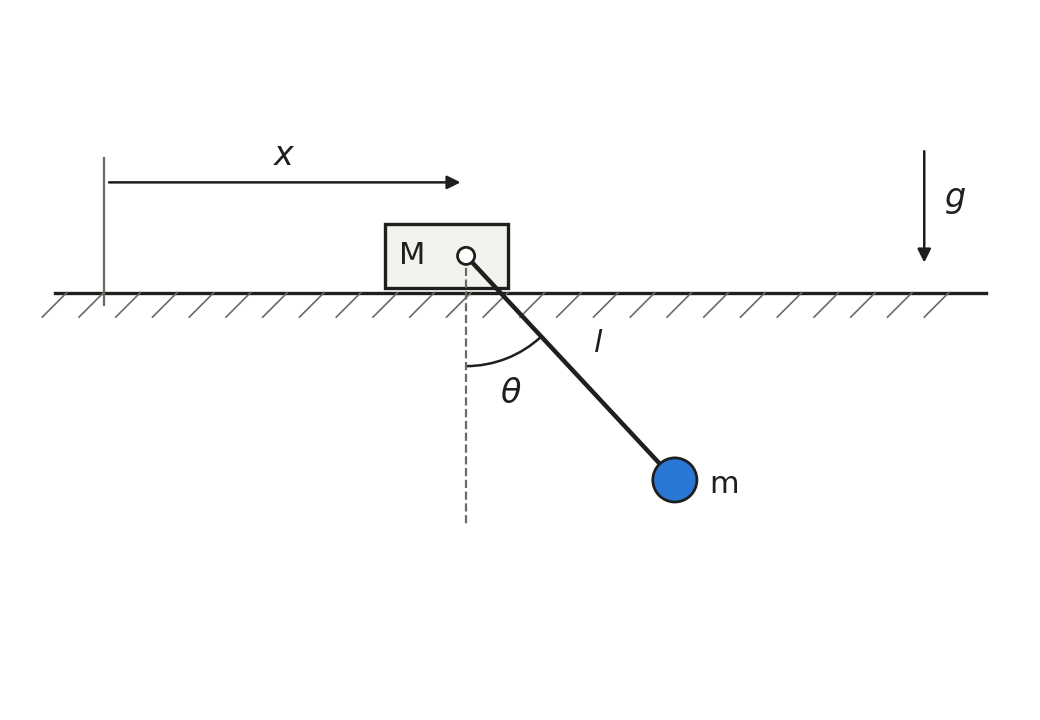
\includegraphics[width=0.52\textwidth]{schematic.png}
\caption{Cart-pole. The cart (mass $M$) slides without friction along the
horizontal track. A massless rigid pole of length $l$, pinned to the cart, carries
a point mass $m$ at its tip.}
\end{figure}

The system moves in the vertical plane. The cart position $x$ is measured along
the track, and the pole angle $\theta$ is measured from the downward vertical,
positive when the bob is on the $+x$ side of the cart. The generalised coordinates are $q = (x,\theta)$. The bob lies at
$(x + l\sin\theta,\; -l\cos\theta)$, and gravity acts in the negative vertical
direction. No other forces act: there is no friction, no damping and no actuation.

\begin{center}
\begin{tabular}{@{}lll@{}}
\toprule
Cart mass & $M$ & \SI{1e-6}{\kilo\gram} \\
Bob mass (point mass at the pole tip) & $m$ & \SI{1}{\kilo\gram} \\
Pole length (massless, rigid) & $l$ & \SI{1}{\metre} \\
Gravity & $g$ & \SI{9.81}{\metre\per\second\squared} \\
\midrule
Initial cart position and velocity & $x_0,\ \dot x_0$ & \SI{0}{\metre},\ \SI{0}{\metre\per\second} \\
Initial pole angle and angular velocity & $\theta_0,\ \dot\theta_0$ & $\pi/2$~rad (horizontal),\ \SI{0}{\radian\per\second} \\
Total simulation time & $T$ & \SI{10}{\second} \\
\bottomrule
\end{tabular}
\end{center}

For reference, the equations of motion are $\mathbf{M}(q)\,\ddot q = \mathbf{F}(q,\dot q)$
with
\begin{equation}
\mathbf{M}(q) = \begin{bmatrix} M+m & ml\cos\theta \\ ml\cos\theta & ml^2 \end{bmatrix},
\qquad
\mathbf{F}(q,\dot q) = \begin{bmatrix} ml\dot\theta^2\sin\theta \\ -mgl\sin\theta \end{bmatrix},
\qquad
\det\mathbf{M} = ml^2\left(M + m\sin^2\theta\right).
\end{equation}
The determinant ranges from $ml^2(M+m)$ when the pole is horizontal down to $ml^2M$
when it is vertical, a ratio of $(M+m)/M \approx 10^{6}$.

Because no horizontal force acts and the system starts at rest, the horizontal
momentum $(M+m)\dot x + ml\dot\theta\cos\theta$ remains zero. The centre of mass
therefore never moves horizontally, and the bob, which carries almost all of the
mass, travels almost vertically. The bob stays at a horizontal position of about
$l$ while the cart slides beneath it between $x \approx 0$ and $x \approx 2l$. The pole passes through the vertical
\Ncross~times in \SI{10}{\second}, first at $t = \Tcross$~s.

\begin{figure}[h]
\centering
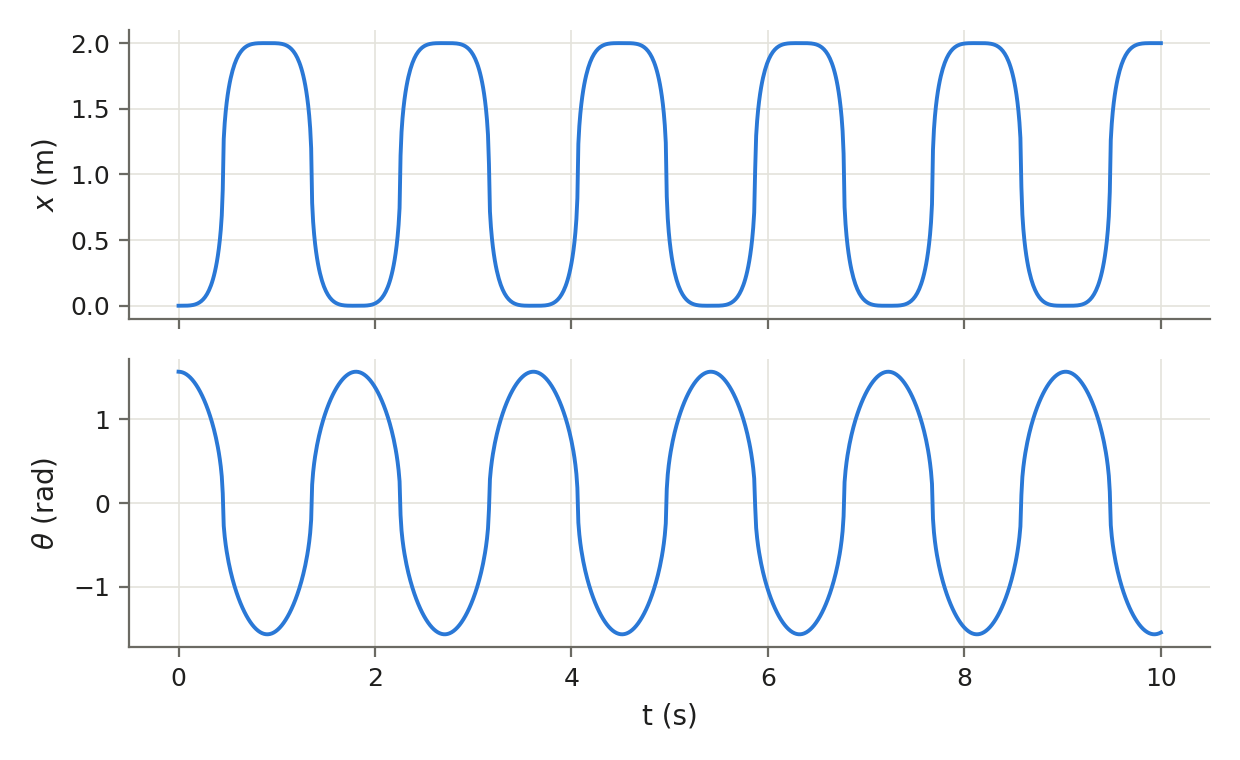
\includegraphics[width=0.78\textwidth]{fig_trajectory.png}
\caption{Reference time histories of the cart position $x$ and the pole angle
$\theta$.}
\end{figure}

\begin{figure}[h]
\centering
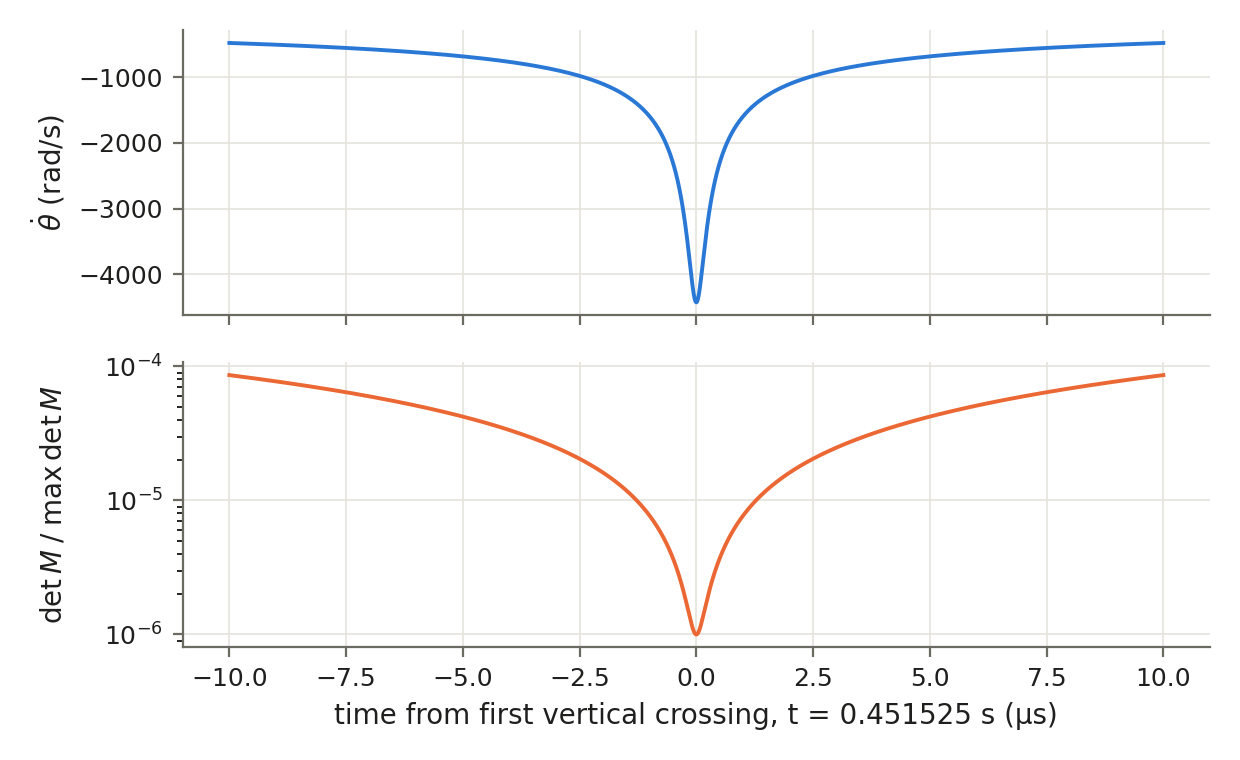
\includegraphics[width=0.78\textwidth]{fig_spike.png}
\caption{Angular velocity, and determinant of the mass matrix relative to its
maximum, in the \SI{20}{\micro\second} around the first vertical crossing. The
spike has a peak of \Peak~rad/s and a full width at half maximum of
\Fwhm~\si{\micro\second}; at \SI{10}{\micro\second} from the crossing $|\dot\theta|$
is still about \Tail~rad/s. The same event recurs at every crossing.}
\end{figure}

\section*{Reference solution}

The reference solution was not produced by any multibody package. The equations of
motion were derived by hand from the Lagrangian, and the $2\times2$ system was
solved in closed form:
\begin{equation}
\ddot x = \frac{m\sin\theta\,(l\dot\theta^2 + g\cos\theta)}{M + m\sin^2\theta},
\qquad
\ddot\theta = -\frac{\sin\theta\,\big((M+m)g + ml\dot\theta^2\cos\theta\big)}{l\,(M + m\sin^2\theta)}.
\end{equation}
The only division is by $M + m\sin^2\theta$, a sum of non-negative terms, so no
cancellation occurs however light the cart becomes. These equations were integrated
with the explicit eighth-order Runge--Kutta method DOP853~\cite{hairer1} as
implemented in SciPy~\cite{scipy}. The relative tolerance was tightened from
$10^{-4}$ to $10^{-13}$ (with absolute tolerance $10^{-2}\times$ the relative
tolerance), and the run at $10^{-13}$ forms the reference. Repeating the ladder with
the implicit Radau IIA method~\cite{hairer2} converges to the same trajectory: at
$10^{-13}$ it agrees with the quadrature solution below to $e =$~\ERadau.

The reference run takes \RefCPU~s on one thread of an Intel Core Ultra~7 255HX
under Windows~11, with Python~\PythonVersion\ and SciPy~\ScipyVersion. This time is
the fastest of three identical runs. Errors at loose tolerances can differ between
SciPy versions; the converged reference does not.

The convergence was checked against a solution obtained without any time
integration. With zero horizontal momentum and conserved energy, the motion reduces
to the quadrature
\begin{equation}
\dot\theta^2 = \frac{2g\,(M+m)(\cos\theta - \cos\theta_0)}{l\,(M + m\sin^2\theta)},
\qquad
x = \frac{ml\,(\sin\theta_0 - \sin\theta)}{M+m},
\end{equation}
which was evaluated, and inverted for $\theta(t)$, in 30-digit arithmetic with
mpmath~\cite{mpmath}. It gives a quarter period of \Qperiod~s. Against this solution
the integrated reference has an error $e$ (defined below) of \Equad, and its
\Ncross~vertical crossings fall within \CrossErr~s of the exact times.

The integrated solution, rather than the quadrature, is used as the reference
because it is produced the way the benchmark asks solutions to be produced, by
time integration of the equations of motion, and because its convergence can be
shown directly. The quadrature depends on conservation laws that hold only for
this force-free, rest-start case, so it serves as an independent check. Since the
two agree to \Equad, five orders of magnitude inside the threshold, the choice does
not affect any score.

\begin{table}[h]
\centering
\small
\begin{tabular}{@{}llrrrr@{}}
\toprule
Integrator & Accelerations & rtol & $e$ vs.\ quadrature & $\max|\Delta E|$ (J) & Evaluations \\
\midrule
DOP853 & closed form & $10^{-4}$ & $7.3\times10^{-3}$ & $4.7\times10^{-3}$ & 10,352 \\
DOP853 & closed form & $10^{-6}$ & $1.1\times10^{-4}$ & $1.4\times10^{-4}$ & 15,923 \\
DOP853 & closed form & $10^{-8}$ & $1.5\times10^{-7}$ & $3.5\times10^{-7}$ & 25,574 \\
DOP853 & closed form & $10^{-10}$ & $2.0\times10^{-9}$ & $2.5\times10^{-9}$ & 43,154 \\
DOP853 & closed form & $10^{-12}$ & $1.2\times10^{-10}$ & $1.4\times10^{-10}$ & 53,240 \\
DOP853 & closed form & $10^{-13}$ & $9.1\times10^{-12}$ & $8.8\times10^{-12}$ & 70,214 \\
Radau & closed form & $10^{-8}$ & $1.2\times10^{-7}$ & $1.4\times10^{-7}$ & 124,746 \\
Radau & closed form & $10^{-10}$ & $7.2\times10^{-10}$ & $9.9\times10^{-10}$ & 386,046 \\
Radau & closed form & $10^{-13}$ & $6.8\times10^{-11}$ & $2.0\times10^{-11}$ & 2,046,293 \\
DOP853 & linear solve & $10^{-8}$ & $1.5\times10^{-7}$ & $3.5\times10^{-7}$ & 25,562 \\
DOP853 & linear solve & $10^{-13}$ & $3.1\times10^{-9}$ & $2.6\times10^{-9}$ & 70,373 \\
\bottomrule
\end{tabular}

\caption{Convergence of the integrated solution as the tolerance is tightened.
$e$ is the benchmark error measured against the 30-digit quadrature solution;
$\max|\Delta E|$ is the largest departure of the mechanical energy from its
initial value. ``Linear solve'' obtains the accelerations by numerically solving
$\mathbf{M}\ddot q = \mathbf{F}$ rather than from the closed form; it stops
improving at about $10^{-9}$, around three hundred times worse than the closed form.}
\end{table}

\begin{figure}[h]
\centering
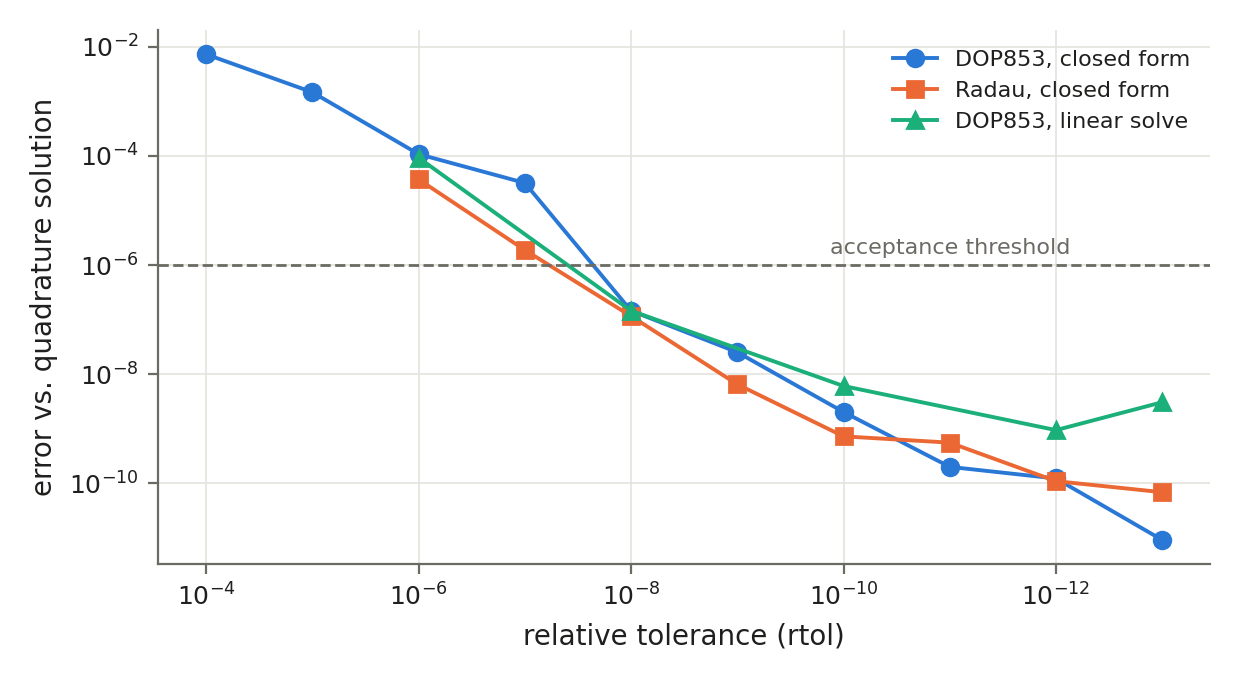
\includegraphics[width=0.78\textwidth]{fig_convergence.png}
\caption{Error against relative tolerance for each integrator and formulation. The
dashed line is the acceptance threshold.}
\end{figure}

The energy appears in the results file only as a secondary check. It converges
together with the trajectory (Table~1), but a small energy drift does not by
itself show that a solution is accurate. The determining check is convergence of
the positions to the quadrature solution.

\section*{Error definition and objective}

Solutions are compared with the reference at the $n = 1001$ sampling times
$t_i = 0.01\,(i-1)$~s, $i = 1,\dots,n$. The error of a simulation is
\begin{equation}
e = \sqrt{\frac{1}{n}\sum_{i=1}^{n}\left[\left(\frac{x(t_i) - x_\mathrm{ref}(t_i)}{l}\right)^{2}
+ \big(\theta(t_i) - \theta_\mathrm{ref}(t_i)\big)^{2}\right]}.
\end{equation}
Absolute rather than relative errors are used because $\theta$ passes through zero.
Velocities are not scored. The \SI{0.01}{\second} grid never lands inside a
spike, so velocity samples would mostly measure timing jitter; an error committed
inside a spike shows up instead as a shift in the timing of $x$ and $\theta$,
which $e$ does capture.

A simulation is considered correct if $e \le 10^{-6}$. The objective is to run the
\SI{10}{\second} simulation in the minimum CPU time while keeping $e$ below this
threshold. Submitters are encouraged to also report the energy drift
$\max_i|E(t_i) - E(0)|$ and, for methods that use them, the number of function
evaluations.

\section*{Results file}

The reference file \texttt{results.txt} has a single header line followed by 1001
rows, one per sampling time, with six whitespace-separated columns:
\begin{enumerate}\setlength{\itemsep}{0pt}
\item time $t$ (s), from 0 to 10 in steps of 0.01;
\item cart position $x$ (m);
\item pole angle $\theta$ (rad), measured from the downward vertical and not wrapped;
\item cart velocity $\dot x$ (m/s);
\item pole angular velocity $\dot\theta$ (rad/s);
\item mechanical energy relative to its initial value, $E(t) - E(0)$ (J).
\end{enumerate}
Submitted results must contain at least the first three columns at the same
sampling times; the remaining columns are optional. The script that generates the
reference solution, the quadrature check and every figure is provided in the
accompanying archive and at
\url{https://github.com/Noah-Parsons/light-cartpole-benchmark}.

\begin{thebibliography}{9}\small
\bibitem{gonzalez}
M.~Gonz\'alez, D.~Dopico, U.~Lugr\'is, and J.~Cuadrado.
A benchmarking system for MBS simulation software: problem standardization and
performance measurement. \emph{Multibody System Dynamics}, 16(2):179--190, 2006.
\bibitem{doublefourbar}
J.~Cuadrado. Double four bar mechanism. IFToMM TC for Multibody Dynamics, Library
of Computational Benchmark Problems.
\url{https://www.iftomm-multibody.org/benchmark/problem/Double_four_bar_mechanism/}.
\bibitem{flyball}
F.~Gonz\'alez and M.~Gonz\'alez. Stiff flyball governor. IFToMM TC for Multibody
Dynamics, Library of Computational Benchmark Problems.
\url{https://www.iftomm-multibody.org/benchmark/problem/Stiff_flyball_governor/}.
\bibitem{hairer1}
E.~Hairer, S.~P.~N{\o}rsett, and G.~Wanner.
\emph{Solving Ordinary Differential Equations I: Nonstiff Problems}.
Springer, 2nd ed., 1993.
\bibitem{hairer2}
E.~Hairer and G.~Wanner.
\emph{Solving Ordinary Differential Equations II: Stiff and Differential-Algebraic
Problems}. Springer, 2nd ed., 1996.
\bibitem{scipy}
P.~Virtanen et al.
SciPy 1.0: fundamental algorithms for scientific computing in Python.
\emph{Nature Methods}, 17:261--272, 2020.
\bibitem{mpmath}
The mpmath development team.
mpmath: a Python library for arbitrary-precision floating-point arithmetic,
version 1.3.0, 2023. \url{https://mpmath.org}.
\end{thebibliography}

\end{document}
